\documentclass[12pt]{article}

\usepackage[utf8]{inputenc}
\usepackage[english]{babel}

\usepackage{amsmath}

\usepackage{mathtools}

\usepackage{amssymb}

\usepackage{stmaryrd}

\usepackage{amsthm}

\usepackage{latexsym}

\usepackage{IEEEtrantools}

\usepackage{eucal}

\usepackage{bbm}

\usepackage[dvipsnames]{xcolor}

\usepackage{tcolorbox}


\usepackage{bussproofs}

\usepackage{graphicx}
\graphicspath{ {./images/} }

\usepackage{stmaryrd}


\usepackage{tikz}

\usetikzlibrary{arrows}



\usepackage{tikz-cd}



%\usepackage{tikzit}

%\input{sample.tikzstyles} Add styles doc here

%\input{sample.tikzdefs}

\usepackage[normalem]{ulem}

\usepackage{hyperref}

\usepackage[dvipsnames]{xcolor}

\definecolor{darkgreen}{RGB}{35, 89, 52}
\definecolor{paleorange}{RGB}{255, 236, 207}

\hypersetup{
	colorlinks=true,
	linkcolor=darkgreen,
	filecolor=magenta,      
	urlcolor=MidnightBlue,
	citecolor=darkgreen,
	pdftitle={Modeling Choice in Co-Design},
	bookmarks=true
}

\title{Modeling Choice in Co-Design}

\author{Marius Furter}

\date{\today}

\usepackage[
backend=bibtex,
style=alphabetic,
citestyle=alphabetic]{biblatex}
\addbibresource{LLCD.bib}

\theoremstyle{definition}

\newtheorem{definition}{Definition}[section]



\theoremstyle{plain} 

\newtheorem{lemma}{Lemma}[section]



\theoremstyle{plain} 

\newtheorem{proposition}{Proposition}[section]



\theoremstyle{plain}

\newtheorem{theorem}{Theorem}[section]


\theoremstyle{plain}

\newtheorem{question}{Question}[section]


\theoremstyle{remark}

\newtheorem{example}{Example}[section]

\newtheorem*{excont}{Example \continuation}
\newcommand{\continuation}{??}
\newenvironment{continueexample}[1]
{\renewcommand{\continuation}{\ref{#1}}\excont[continued]}
{\endexcont}


\theoremstyle{remark}

\newtheorem{remark}{Remark}[section]

\newcommand{\zuz}[1]{%

	\begin{tikzpicture}[#1]%

	\draw[semithick, line cap = round, line join = round] (-0.3ex,0.35ex) -- (0.5ex,0.35ex);

	\draw[semithick, line cap = round, line join = round] (0.5ex,0.35ex) -- (0.5ex,-0.5ex);

	\draw[semithick, line cap = round, line join = round] (0.5ex,-0.5ex) -- (1.5ex,-0.5ex);

	\draw[semithick, line cap = round, line join = round] (0,0) -- (1ex,0);%

	\draw[semithick, line cap = round, line join = round] (1ex,0) -- (1ex,-0.85ex);

	\draw[semithick, line cap = round, line join = round] (1ex,-0.85ex) -- (1.8ex,-0.85ex);

	\end{tikzpicture}%

} 



\renewcommand\qedsymbol{\zuz{scale=1.5}}

\newcommand{\mc}[1]{\mathcal{#1}}

\newcommand{\maybe}{\mathsf{Maybe}}

\newcommand{\either}{\mathsf{Either}}

\newcommand{\both}{\mathsf{Both}}

\newcommand{\sub}{\subseteq}

\newcommand{\Hom}{\text{Hom}}

\newcommand{\im}{\text{im}}

\newcommand{\id}{\text{id}}

\newcommand{\low}{\mathsf{L}}

\newcommand{\upper}{\mathsf{U}}

\newcommand{\ac}{\mathsf{A}}

\newcommand{\true}{\mathtt{true}}
\newcommand{\false}{\mathtt{false}}

\newcommand{\upc}[1]{{\uparrow #1}}
\newcommand{\lwc}[1]{{\downarrow #1}}

\makeatletter
\def\slashedarrowfill@#1#2#3#4#5{%
	$\m@th\thickmuskip0mu\medmuskip\thickmuskip\thinmuskip\thickmuskip
	\relax#5#1\mkern-7mu%
	\cleaders\hbox{$#5\mkern-2mu#2\mkern-2mu$}\hfill
	\mathclap{#3}\mathclap{#2}%
	\cleaders\hbox{$#5\mkern-2mu#2\mkern-2mu$}\hfill
	\mkern-7mu#4$%
}
\def\rightslashedarrowfill@{%
	\slashedarrowfill@\relbar\relbar\mapstochar\rightarrow}
\newcommand\xslashedrightarrow[2][]{%
	\ext@arrow 0055{\rightslashedarrowfill@}{#1}{#2}}
\makeatother


\begin{document}

\maketitle

\begin{abstract}
	Write this
\end{abstract}
\newpage
\tableofcontents
\newpage

\section{Introduction}
Living life involves making choices. Before a choice is made, a set of unrealized options lies dormant. Making a choice involves collapsing this set to a single outcome. This collapse may occur in several ways. On the one extreme, we may be in full control of which option is realized: We are able to freely choose a desired outcome. On the other extreme, we may be powerless to steer the collapse: A choice is forced upon us.

Choice is relevant in any discipline that involves a multiplicity of potential outcomes. In computer science, for example, choice is used to describe program specifications \cite{Martin2007,Morris2004}. Here the choice is between possible outputs of non-deterministic code. Free choice corresponds to the code behaving in the programmers best interest, while forced choice describes an uncertainty of outcome. These two modes are personified by an angel choosing on behalf of the programmer in the first case, while a demon chooses in the latter.

Choice also arises whenever one requires coordination between agents. Alice might only be able to guarantee a range of outcomes to Bob. This is weaker than guaranteeing a specific outcome. On the other hand, Alice may be able to offer Bob a free choice between a set of outcomes. This is stronger than offering a single outcome. We see that allowing for free and forced choices expands the space of possible interactions between Alice and Bob.

In engineering too, choices abound. A team can freely choose a specific motor from a catalog of options. On the other hand, a team might only be able to guarantee that their design will fulfill one of several properties: Their robot will either be able to move fast or carry a lot of weight, but they aren't specifying which. Such uncertainty in outcome has ramifications for other teams working on the project. 

Questions of coordination between teams are addressed in the Co-Design framework \cite{Censi2015}. However, the original framework does not include a way to express free and forced choices. Here we aim to extend the framework in a way that does. 

\subsection{Goals}
This report aims to succinctly describe how to model free and forced choice within the Co-Design framework. Additionally, it will highlight avenues for future exploration. Ideally, it could serve as a starting point for anyone seeking to make further contributions to this topic.

\subsection{Structure}

\section{A Brief Introduction to Co-Design}
We begin by providing a short introduction to the Co-Design framework established in \cite{Censi2015}. This will also serve to fix the conventions we will be using throughout. \\

In Co-Design we consider resources that can be used to achieve functionalities. For example, we might consider different types of motor as resources, with the power output they provide as functionalities. If a resource $r$ can be used to provide functionality $f$ we say that the pair $(r,f)$ is feasible. Continuing our example, if motor $A$ is capable of ouputting \mbox{2 kW} then we would mark $(A,\text{2 kW})$ as feasible.

It can occur that certain resources or functionalities imply others. If motor $A$ can provide \mbox{2 kW}, it should also be able to provide \mbox{1 kW}. We will indicate this by writing $2 \text{ kW} \rightarrow 1 \text{ kW}$. Hence, our sets of resources and functionalities posses additional structure: They are preorders. Consequently, we want our notion of feasibility to take this structure into account. This leads to the concept of \emph{feasibility relation}. We will make these ideas precise in what follows.

\subsection{Resource and Functionality Preorders}

We model resources and functionalities using preordered sets, which will be formally introduced shortly. We interpret an element $a$ of the preorder as the guarantee ``I can provide $a$''. We put an arrow $a \shortrightarrow b$ whenever being able to provide $a$ implies being able to provide $b$. This is best illustrated with an example.

\begin{example}(Money as Resources)\label{ex:money}
	The set $\mathbb{N} := \{0,1,2,\ldots \}$ with the order relation $a \shortrightarrow b \Leftrightarrow a \geq b$ can be used to describe money (of a single currency, say dollars) as a resource. The element $a$ represents being able to provide $a$ dollars, while $a \shortrightarrow b$ means that if you can provide $a$ dollars, you can also provide $b$ dollars. For example, $3 \shortrightarrow 1$ signifies that if we could pay 3 dollars, we also possess the purchasing power of 1 dollar. Observe that being able to transform $3 \shortrightarrow 1$ presupposes that people are willing to accept $3$ dollars in lieu of $1$ dollar. This hypothesis is system relative. For example, a vending machine might only accept bills of low denomination. So in this case one might well not have $50 \shortrightarrow 1$.
\end{example}

Returning to the general theory, we observe that the preorder axioms precisely describe how we would like the relation $a \shortrightarrow b$ to behave.

\begin{definition}(Preorder)\label{def:preorder}
	A \emph{preorder} is a set with a binary relation $R \sub A \times A$ satisfying reflexivity (r) and transitivity (t):
	\begin{itemize}
		\item[(r)] $(a,a) \in R$ for all $a \in A$,
		\item[(t)] if $(a,b) \in R$ and $(b,c) \in R$, then $(a,c) \in R$.
	\end{itemize}
	Usually we write the pair $(a,b)$ using an infix symbol. In our case, $a \shortrightarrow b$ means $(a,b)$ is part of the relation $R$.
\end{definition}

Using our infix notation, the two axioms become 
\begin{itemize}
	\item[(r)] $a \shortrightarrow a$ for all $a$,
	\item[(t)] $a \shortrightarrow b$ and $b \shortrightarrow c$ imply $a \shortrightarrow c$.
\end{itemize}  
In other words, for each resource $a$, being able to provide $a$ implies being able to provide $b$. Further, if being able to provide $a$ implies being able to provide $b$, and being able to provide $b$ implies being able to provide $c$, then being able to provide $a$ should imply being able to provide $c$. \\

Everything that has been said here applies equally to functionalities. In fact, what we view as resources and functionalities is relative to the process we are considering. When I purchase a candy bar from a vending machine, the dollar I spend is the resource, and the candy bar the functionality. When I eat the candy bar to gain energy, the candy bar has become the resource.

\begin{tcolorbox}[title=Resources and Functionalities, colframe=Apricot, colback = paleorange, coltitle = Sepia]
	Resources and functionalities are modeled by preorders. An element $a$ in the preorder expresses the guarantee \emph{``I can provide $a$''}. An arrow $a \shortrightarrow b$ means \emph{``being able to provide $a$ implies being able to provide $b$''}. 
\end{tcolorbox}

\begin{remark}
	There are some fine points here that may be skipped on a first reading. Observe that our guarantee does not specify who we are providing $a$ to. The recipient might be another agent or our (future) selves. More generally, there are other interpretations we could give the elements and arrows in our preorders. Two of them are discussed in the following boxes. Ultimately, these just provide a different flavor to the theory. Our preferred interpretation fits best with thinking about choice.
\end{remark}

\begin{tcolorbox}[title= Functionality Interpretation]
	 Following the logic of Co-Design, a resource is determined by the functionality it can provide. From this perspective, we could alternatively set $a \shortrightarrow b$ whenever $a$ provides at least the same level of functionality as $b$ does. In this case, in terms of the functionality on offer, being able to provide $a$ does implies being able to provide $b$. Conversely, if being able to provide $a$ implies being able to provide $b$, then $a$ must offer at least the same level of functionality as $b$. This shows that the two interpretations align.
\end{tcolorbox}

\begin{tcolorbox}[title= Transformation Interpretation]
	We could also interpret $a \shortrightarrow b$ as meaning that we can freely and instantly transform $a$ into $b$. If $a$ freely transforms into $b$, then being able to provide $a$ implies being able to provide $b$. Conversely, if being able to provide $a$ implies being able to provide $b$, then given $a$, we should be able to provide $b$. This can be seen as a free transformation of $a$ into $b$.
\end{tcolorbox}


\subsection{Feasibility Relations}
Given a preorder of resources $\mc{R}$ and a preorder of functionalities $\mc{F}$, a feasibility relation $\Phi: \mc{R} \xslashedrightarrow{} \mc{F}$ between them expresses which functionalities I am able to obtain from which resources. We write $\Phi(r,f) = \mathtt{true}$ to indicate that $f$ can be obtained from $r$.

\begin{example}\label{ex:groceries}
	Consider buying groceries. Our resources $\mc{R}$ will be money as in Example \ref{ex:money}. The possible groceries we can buy are the functionalities $\mc{F}$. The feasibility relation $\Phi: \mc{R} \xslashedrightarrow{} \mc{F}$ will describe what groceries we can purchase given a specific amount of cash. For example, a $\mathtt{carrot}$ might cost $1\$$. Hence, $\Phi(1\$,\mathtt{carrot}) = \mathtt{true}$. On the other hand, $\Phi(0\$, \mathtt{carrot}) = \mathtt{false}$, since we can't get a $\mathtt{carrot}$ without paying anything. Suppose now that a $\mathtt{bag\ of\ carrots}$ costs $3\$$. This means $\Phi(3\$,\mathtt{bag\ of\ carrots}) = \mathtt{true}$. Observe that also $\Phi(3\$,\mathtt{carrot}) = \true$ should hold. Either we can pick up a single carrot in the store and pay for it with $3\$$, or we could buy the whole bag for $3\$$ and this would also give us a single $\mathtt{carrot}$. 
	
	This shows that feasibility interacts with the implication arrows we have for the resources and functionalities. In our example,
	$$3\$ \shortrightarrow 1\$ \text{ and } \Phi(1\$, \mathtt{carrot}) = \true  \text{ implied } \Phi(3\$, \mathtt{carrot}) = \true.$$ 
	Similarly, 
	$$\mathtt{bag\ of\ carrots} \shortrightarrow \mathtt{carrot}  \text{ and } \Phi(3\$,\mathtt{bag\ of\ carrots}) = \mathtt{true} $$ 
	implied that $\Phi(3\$,\mathtt{carrot}) = \true.$
\end{example}

The interaction we observed between arrows and feasibility justifies the formal definition of a feasibility relation.

\begin{definition}[Feasibility Relation]\label{def:feasibility}
	Given preorders $\mc{R}$ and $\mc{F}$, a \emph{feasibility relation} $\Phi: \mc{R} \xslashedrightarrow{} \mc{F}$ is a relation $\Phi \sub \mc{R} \times \mc{F}$ such that
	\begin{itemize}
		\item[(i)] if $r \shortrightarrow s$ in $\mc{R}$ and $(s,f) \in \Phi$, then $(r,f) \in \Phi$,
		\item[(ii)] if $f \shortrightarrow g$ in $\mc{F}$ and $(r,f) \in \Phi$, then $(r,g) \in \Phi$.
	\end{itemize}
	If $(r,f) \in \Phi$ we write $\Phi(r,f) = \true$ and say that $\Phi(r,f)$ holds.
\end{definition}

In other words, a feasibility relation is a relation from $\mc{R}$ to $\mc{F}$ that is downward closed with respect to free transformations in $\mc{R}$ and upward closed with respect to free transformations in $\mc{F}$. We will often draw internal diagrams of feasibility relations as in Figure \ref{fig:internal feas}. We put an arrow between an $r \in \mc{R}$ and $f \in \mc{F}$ iff $\Phi(r,f) = \true$. The arrows coming from $\Phi$ can be thought of the transformations that $\Phi$ enables. Observe that the closure conditions in Definition \ref{def:feasibility} mean that the arrows coming from $\Phi$ are transitively closed with respect to the internal arrows in $\mc{R}$ and $\mc{F}$: If there is a path from an $r \in \mc{R}$ to an $f \in \mc{F}$ following any type of arrow, then we also have a direct arrow between $r$ and $f$ coming from $\Phi$.

\begin{continueexample}{ex:groceries}
	We can now formally implement our example of grocery shopping. Recall that our resource preorder $\mc{R}$ consists of money, while our functionality preorder $\mc{F}$ describes groceries we can purchase. Figure \ref{fig:internal feas} shows part of an internal diagram of a feasibility relation $\Phi: \mc{R} \xslashedrightarrow{} \mc{F}$. The blue arrows indicate the feasible pairs. For example, $$\Phi(3\$,\mathtt{bag\ of\ carrots}) = \true.$$ It is worth contemplating why $\Phi$ satisfies the monotonicity conditions presented in Definition \ref{def:feasibility}.
	
	\begin{figure}
		\centering
		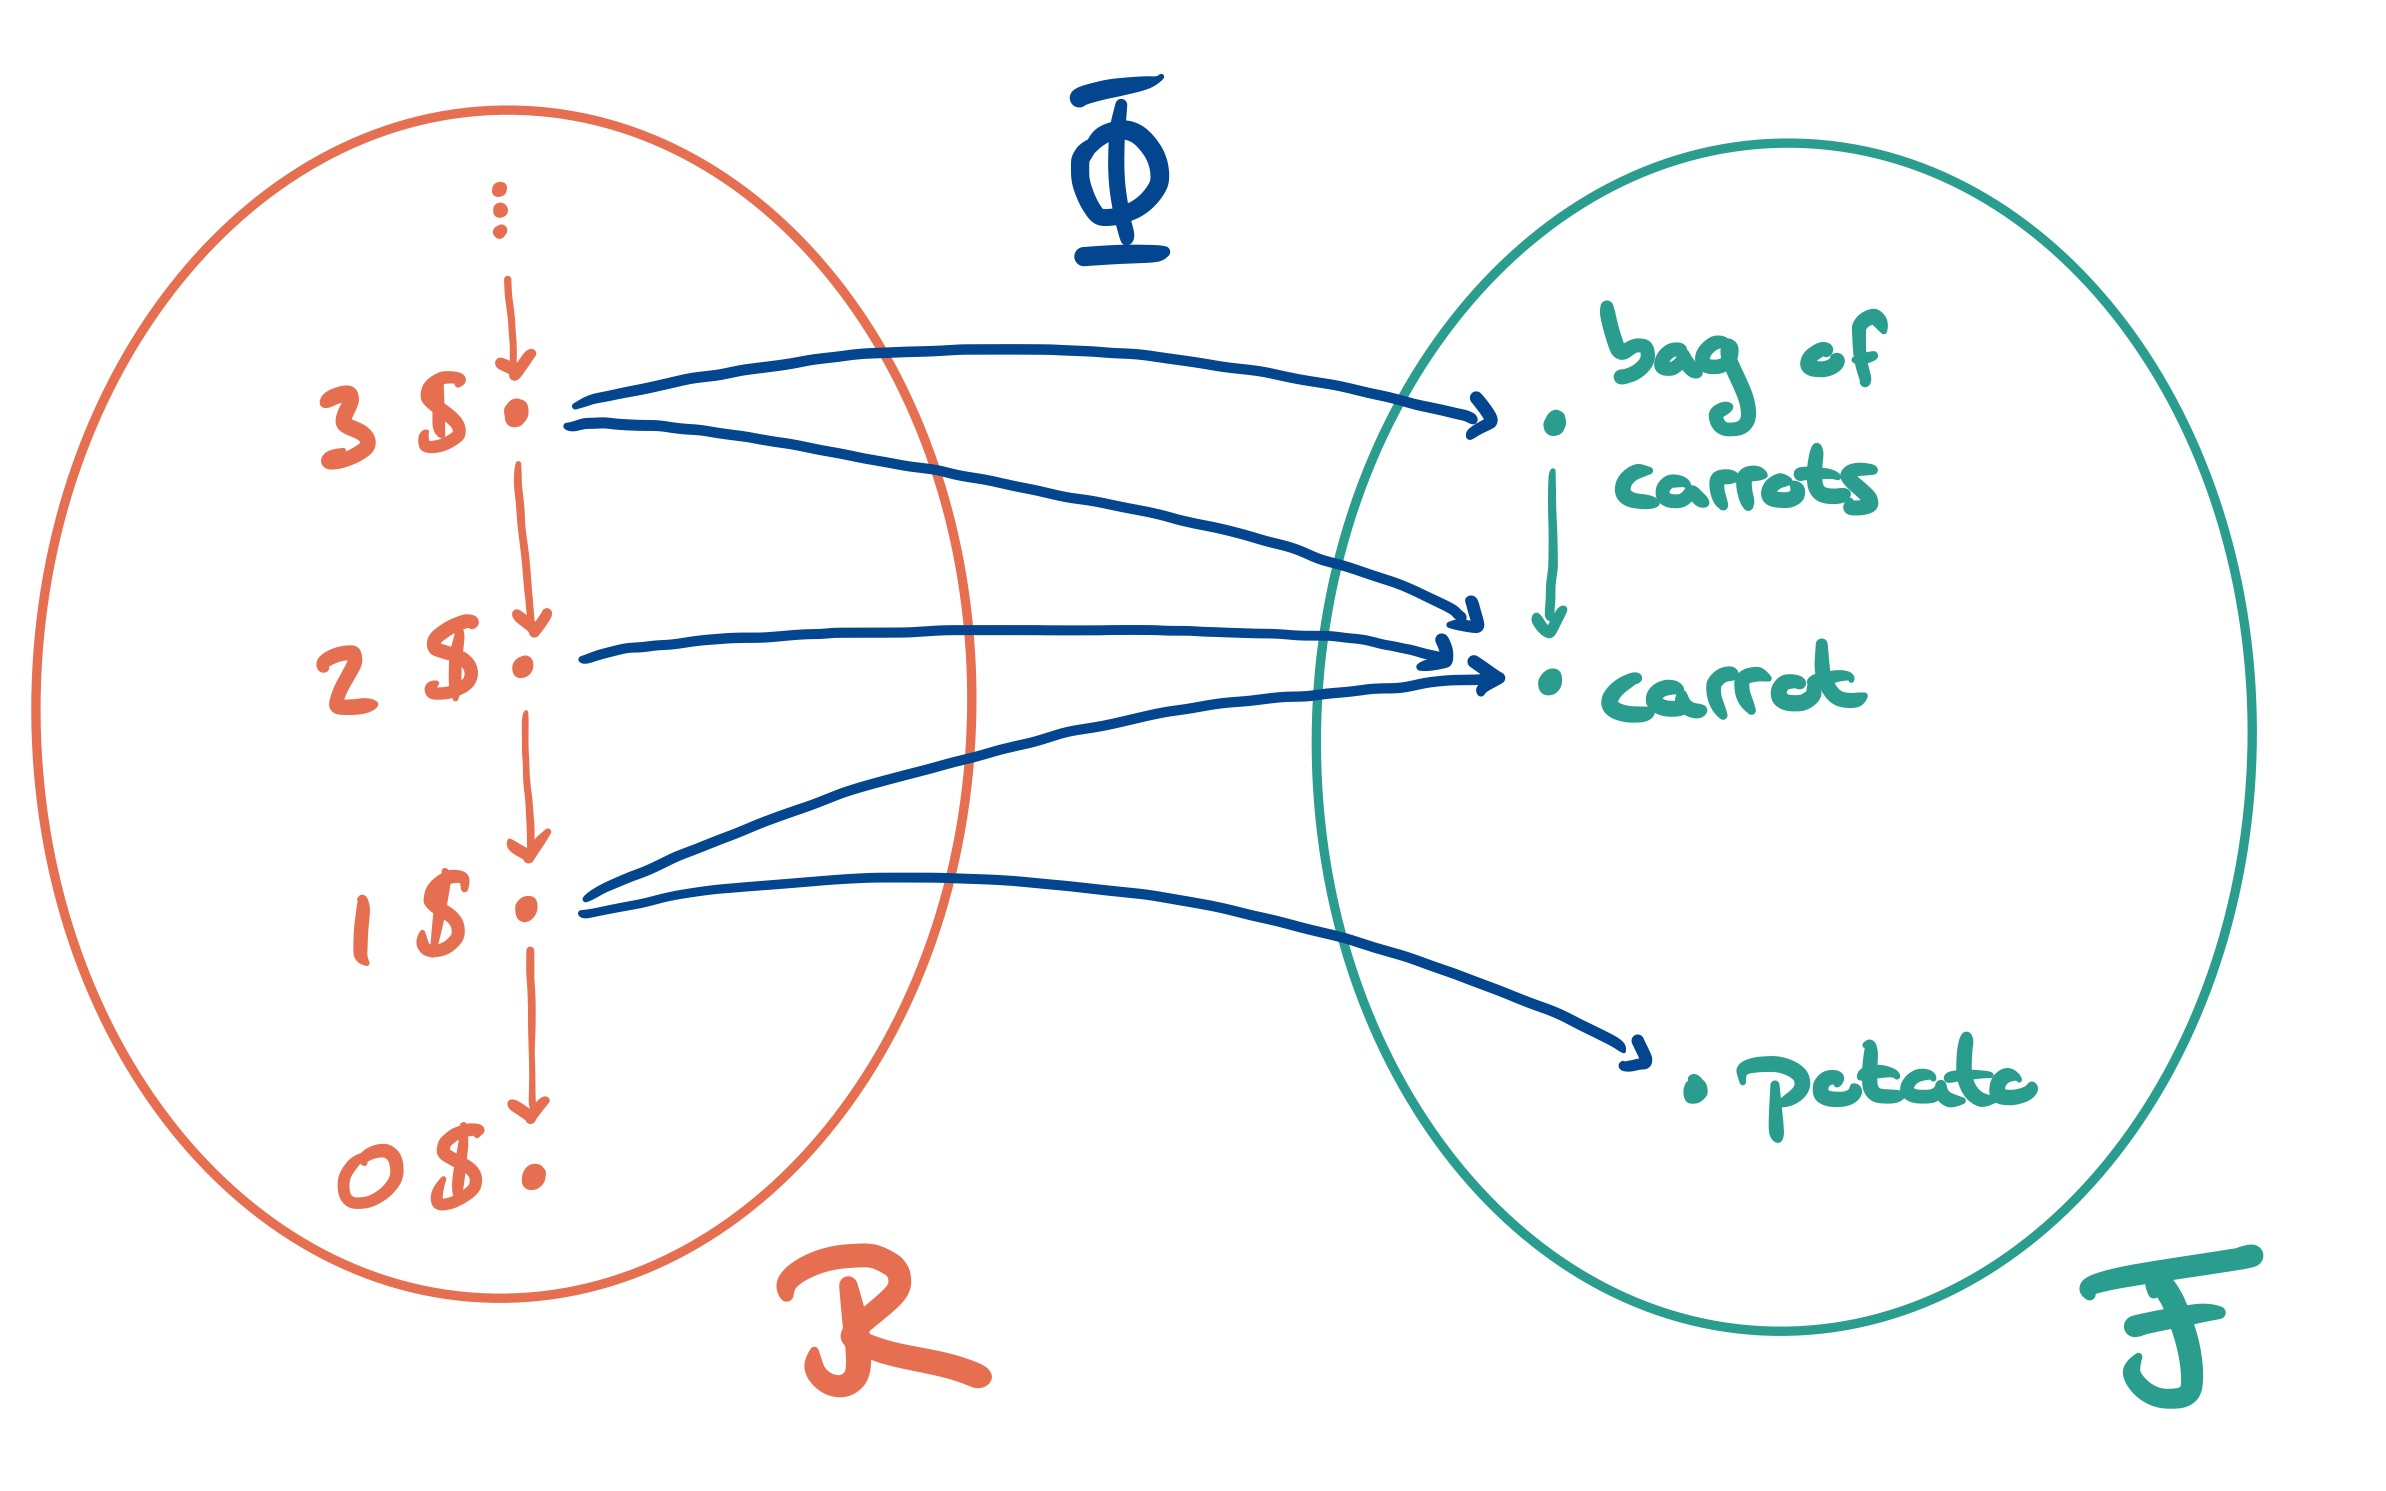
\includegraphics[width=350pt]{images/ex_groceries}
		\caption{Internal diagram of a feasibility relation $\Phi: \mc{R} \xslashedrightarrow{} \mc{F}$.}
		\label{fig:internal feas}
	\end{figure}
	
\end{continueexample}

We could have also defined feasibility relations as special types of monotone maps. For this we need to introduce several concepts.

\begin{definition}
	Let $\mathsf{Bool}$ denote the preorder generated by $\{\false \rightarrow \true\}$. Explicitly, $\mathsf{Bool}$ contains the arrows $\false \shortrightarrow \false$, $\false \shortrightarrow \true$, and $\true \rightarrow \true$.
\end{definition}

\begin{definition}[Opposite Preorder]
	Given a preorder $(\mc{P},\shortrightarrow)$, we define its \emph{opposite preorder} $\mc{P}^\text{op}$ to be the preorder that is obtained by reversing all the arrows in $\mc{P}$. That is, we set $a \shortrightarrow b$ in $\mc{P}^\text{op}$ if and only if $b \shortrightarrow a$ in $\mc{P}$. 
\end{definition}

\begin{definition}[Product of Preorders]
	Let $\mc{P}$ and $\mc{Q}$ be preorders. Their \emph{product} $\mc{P} \times \mc{Q}$ consists of all pairs $(p,q)$ where $p \in \mc{P}$ and $q \in \mc{Q}$ where we set $(p,q) \shortrightarrow (p',q')$ if and only if $p \shortrightarrow p'$ in $\mc{P}$ and $q \shortrightarrow q'$ in $\mc{Q}$.
\end{definition}

\begin{definition}[Monotone Map]
	Let $\mc{P}$ and $\mc{Q}$ be preorders. A function $f: \mc{P} \rightarrow \mc{Q}$ is called \emph{monotone} if it preserves the order in $\mc{P}$. That is, whenever $a \shortrightarrow b$ in $\mc{P}$, we have $f(a) \shortrightarrow f(b)$ in $\mc{Q}$.
\end{definition}

\begin{lemma}
	There is a one-to-one correspondence between feasibility relations $\Phi: \mc{R} \xslashedrightarrow{} \mc{F}$ and monotone maps $\mc{R}^\text{op} \times \mc{F} \rightarrow \mathsf{Bool}$.
\end{lemma}
\begin{proof}
	Given a feasibility relation $\Phi: \mc{R} \xslashedrightarrow{} \mc{F}$ as defined in Definition \ref{def:feasibility}, we obtain a function $F: \mc{R}^\text{op} \times \mc{F} \rightarrow \mathsf{Bool}$ by sending $(r,f) \mapsto \true$ if and only if $(r,f) \in \Phi$. Conditions (i) and (ii) of Definition \ref{def:feasibility} say that this function is monotone. Conversely, given a monotone map $F: \mc{R}^\text{op} \times \mc{F} \rightarrow \mathsf{Bool}$, we can obtain a relation $\Phi$ by setting $(r,f) \in \Phi$ if and only if $F(r,f) = \true$. The monotonicity of this function implies that $\Phi$ satisfies conditions (i) and (ii). It is apparent that these processes are inverse to one another.
\end{proof}

\begin{tcolorbox}[title=Feasibility Relations, colframe=Apricot, colback = paleorange, coltitle = Sepia]
	A feasibility relation $\Phi: \mc{R} \xslashedrightarrow{} \mc{F}$ expresses which functionalities in $\mc{F}$ can be obtained from which resources in $\mc{R}$. We write $\Phi(r,f) = \mathtt{true}$ to indicate that $f \in \mc{F}$ can be obtained from $r \in \mc{R}$. The relation $\Phi$ needs to satisfy the two monotonicity conditions in Definition \ref{def:feasibility} which can be concisely expressed by saying the $\Phi$ is a monotone map $\mc{R}^\text{op} \times \mc{F} \rightarrow \mathsf{Bool}$.
\end{tcolorbox}

\section{Choice between Resources}
We will now extend what we've seen so far to encompass choice and uncertainty. What is meant by these terms is best illustrated with an example.

\begin{example}[Menu Options]\label{ex:menu}
	In a restaurant we might see the following menu options.
	\begin{itemize}
		\item Coffee or tea (customer choice)
		\item Asparagus or beetroot soup (depending on availability)
	\end{itemize}
	In the first case, we as customers are given the choice between coffee or tea. In the second, it is chosen for us which soup we will get, depending on what the cooks have available. From our perspective as customers, this represents an uncertainty. In both cases, however, we will end up with exactly one of the options.
\end{example}

We might refer to the two modes of choice presented in Example \ref{ex:menu} as \emph{internal choice} and \emph{external choice}, respectively. Alternatively, we could call them \emph{choice} and \emph{uncertainty}, or \emph{free} and \emph{forced} choice. Regardless of the names we choose, the terms are relative to which perspective we are taking. If we look through the eyes of the restaurant, the customer choice of coffee or tea is external, while the choice of soup is internal.

\subsection{Choice Connectives}
To formalize the two modes of choice described above, we introduce two connectives, denoted  $\sqcup$ and $\sqcap$, respectively. Because the distinction between what is internal and external is relative to what perspective we are taking, we will hold off on generally fixing which symbol denotes which mode of choice. Instead, we will always indicate what the interpretation should be in each specific case. \\

For the moment, fix $\sqcap$ as free choice and $\sqcup$ as forced choice. Hence, to  denote a free choice from a set $A$ we write $\bigsqcap_{a \in A} a$, while for a forced choice from a set $B$ we write $\bigsqcup_{b \in B} b$. We will now see how such choices should interact with the free transformations we have in a resource preorder, as well as each other.

\subsubsection{Interaction of Choice with Free Transformations}\label{sec:intr free}
Let $\mc{R}$ be a preorder of resources. If we have a free choice of any $a \in A$, then we can freely transform that choice into any specific $a \in A$ by making the corresponding choice. For example, if I have a choice between coffee or tea, I implicitly have coffee, and I implicitly have tea. In other words, I can downgrade any choice I get to make to the certainty of having one of the items I get to choose from. Formally, we have 
\begin{equation}\label{eq:meet 1}
	\bigsqcap_{a \in A} a \shortrightarrow a, \quad \forall a \in A.
\end{equation}

Now suppose we can freely obtain all $a$ in a set $A$ from a fixed resource $t$. In that case, having $t$ means implicitly having a free choice between any $a \in A$. For any $a$ you end up choosing, there is a free way to get that $a$ from $t$. Formally,
\begin{equation}\label{eq:meet 2}
	\forall a \in A : t \shortrightarrow a  \quad \Rightarrow \quad t \shortrightarrow 	\bigsqcap_{a \in A} a.
\end{equation}

Dually, if I have any $b \in B$ for certain, I can freely transform it into a forced choice among all $b \in B$. For example, having asparagus soup also implicitly means you have asparagus or beetroot soup (depending on availability). In other words, we can downgrade the certainty of having a specific $b \in B$ to the uncertainty of having some $b \in B$. Formally, this becomes
\begin{equation}\label{eq:join 1}
b \shortrightarrow \bigsqcup_{b \in B} b, \quad \forall b \in B.
\end{equation}

Finally, suppose that for every $b \in B$ there is a free transformation to a fixed resource $t$. In that case, if someone chooses an arbitrary $b \in B$ for you, you can still freely obtain $t$ using the corresponding free transformation. Hence,
\begin{equation}\label{eq:join 2}
\forall b \in B : b \shortrightarrow t  \quad \Rightarrow \quad  \bigsqcup_{b \in B} b \shortrightarrow t.
\end{equation}


Mathematically, (\ref{eq:meet 1}) and (\ref{eq:meet 2}) mean that $\sqcap$ is the \emph{meet} over $a \in A$, while (\ref{eq:join 1}) and (\ref{eq:join 2}) show that $\sqcup$ is the \emph{join} over $b \in B$.

\subsubsection{Mutual Interaction of the Two Modes of Choice}\label{sec:intr self}
We now look at how the two connectives should interact with each other. First we consider the finite case. For simplicity we write 
$$\bigsqcap_{x \in \{a,b\}} x =: a  \sqcap b,$$
$$\bigsqcup_{x \in \{a,b\}} x =: a  \sqcup b.$$

Suppose we have a series of choices given by $a \sqcap (b \sqcup c)$. This means we get to freely choose between getting $a$ for certain, or between the uncertainty of getting $b$, or $c$. In this scenario, we can always guarantee $a$ if we want, but we are uncertain whether we will get $b$ or $c$, if we don't choose $a$. Compare this with the series of choices given by $(a \sqcap b) \sqcup (a \sqcap c)$. Here too we can always guarantee the $a$, but are uncertain whether we will get $b$ or $c$, if we don't choose $a$. In fact, in terms of which resources we can guarantee, the two formulations are equivalent from our perspective. Hence, we can assume the following distributive law $$a \sqcap (b \sqcup c) \cong (a \sqcap b) \sqcup (a \sqcap c).$$

Dually, we can compare $a \sqcup (b \sqcap c)$ with $(a \sqcup b) \sqcap (a \sqcup c)$. In the first expression we are uncertain whether we will get $a$, or a free choice between $b$ and $c$. This means that if we don't get $a$, we can guarantee either $b$ or $c$. This is also the case in the second expression. Hence, we may assume the distributive law $$a \sqcup (b \sqcap c) \cong (a \sqcup b) \sqcap (a \sqcup c).$$

More generally, these equalities should also hold for the infinite case. The statement of the infinite distributive law is more complicated: For any doubly indexed family of elements $\{b_{j,k} : j \in J, k \in K_j\}$ of $\mc{R}$ we have
\begin{equation}\label{eq:meet dist}
	\bigsqcap_{j \in J} \left( \bigsqcup_{k \in K_j} b_{j,k} \right) \cong \bigsqcup_{f \in F} \left( \bigsqcap_{j \in J} b_{j,f(j)} \right),
\end{equation}
where $F$ is the set of all choice functions choosing for each index $j \in J$ some index $f(j) \in K_j$.

Suppose we are presented with a choice of the form $\bigsqcap_{j \in J} \left( \bigsqcup_{k \in K_j} b_{j,k} \right)$. Then we can guarantee $\bigsqcup_{k \in K_j} b_{j,k} $ for any $j \in J$ we choose. That is we can guarantee uncertainty only between the $b_{j,k}$ for one specific $j$ of our choice. Now consider $\bigsqcup_{f \in F} \left( \bigsqcap_{j \in J} b_{j,f(j)} \right)$. Here, some $f \in F$ is chosen for us. We then get to chose freely between the $b_{j,f(j)}$ for that fixed $f$. Hence we still have uncertainty among a set of $b_{j,k}$ for a $j$ of our choice. Moreover, $f$ picks precisely one $k = f(j)$ among all $k \in K_j$, so the set of $b_{j,k}$ for which there is uncertainty remains the same in both cases.

We can also formulate the dual distributive law
\begin{equation}
\bigsqcup_{j \in J} \left( \bigsqcap_{k \in K_j} b_{j,k} \right) \cong \bigsqcap_{f \in F} \left( \bigsqcup_{j \in J} b_{j,f(j)} \right),
\end{equation}
which happens to be equivalent to (\ref{eq:meet dist}) provided all both $\bigsqcap_{a \in A}$ and $\bigsqcup_{a \in A}$ exist for any subset $A \sub \mc{R}$.

\subsubsection{Laws for the Choice Connectives}
We have seen that the choice connectives $\sqcap$ and $\sqcup$ on a resource preorder should behave like meets and joins over arbitrary subsets of $\mc{R}$. Moreover, they should distribute over one another, even in the infinite case. Hence, any structure that we use to model choice should be a completely distributive lattice. Conversely, such a model shouldn't satisfy any other laws that are not implied by our desired laws. This leads us to consider the free distributive lattice on $\mc{R}$ to model choice. 

There are several notions of free distributive lattice one could use, depending on what set of maps one is interested in. We will follow \cite{Morris2004} which shows that the upper sets of lower sets of $\mc{R}$, denoted $\upper(\low(\mc{R}))$ satisfy the following universal property:
\begin{quote}
	There is an order embedding $i: \mc{R} \hookrightarrow \upper(\low(\mc{R}))$, such that for any monotone function $f: \mc{R} \rightarrow M$ into a completely distributive lattice $M$, there is a unique complete homomorphisms $u: \upper(\low(\mc{R})) \rightarrow M$ (preserving arbitrary meets and joins) satisfying $u \circ i = f$.
\end{quote}

In particular, if we put any completely distributive choice structure $M$ on $\mc{R}$, there will be a unique map from $u: \upper(\low(\mc{R})) \rightarrow M$, preserving choices. 

\subsection{The Upper-Lower Model}\label{sec:upper-lower model}
In this section we introduce and interpret the choice structure on a resource preorder $\mc{R}$ given by $\upper(\low(\mc{R}))$. First, we will show how to use the upper-lower construction as a purely formal tool that realizes the desired properties we derived in Sections \ref{sec:intr free} and \ref{sec:intr self}. Then, we will reconstruct the upper-lower model by giving an interpretation to the sets appearing therein. This will include deriving the corresponding laws based on that interpretation. The fact that both approaches agree suggests that we have chosen a good model.

\subsubsection{Formally using the Upper-Lower Model}
We begin by describing $\upper(\low(\mc{R}))$ in greater detail. We again fix $\sqcap$ as free choice and $\sqcup$ as forced choice. First, we define the lattice of lower sets.

\begin{definition}[Lower Sets]
	Let $(P,\shortrightarrow)$ be a preorder. A subset $L \sub P$ is a lower set, iff for any $l \in L$, $x \shortrightarrow l$ implies $x \in L$. The set of lower sets of $P$, ordered by inclusion is denoted by $\low(P)$. 
\end{definition}

\begin{lemma}
	For any preorder $P$, $\low(P)$ is a completely distributive lattice with meets given by set intersection and joins by set union.
\end{lemma}

\begin{definition}[Lower Closure]
	Given a subset $A \sub P$, its lower closure is the lower set given by $$\downarrow A := \{x \in P: x \shortrightarrow a \text{ for some a } \in A\}.$$
\end{definition} 

\begin{lemma}
	For any preorder $P$, we can embed $i: P \hookrightarrow \low(P)$ by taking lower closures $p \mapsto \downarrow \{p\}$. This map is injective and satisfies $p \shortrightarrow q \Leftrightarrow i(p) \sub i(q).$ 
\end{lemma}

Dually, we can make the same definitions for upper sets.

\begin{definition}[Upper Sets]
	Let $(P,\shortrightarrow)$ be a preorder. A subset $U \sub P$ is an upper set, iff for any $u \in U$, $u \shortrightarrow x$ implies $x \in U$. The set of upper sets of $P$, ordered by containment is denoted by $\upper(P)$. 
\end{definition}

\begin{lemma}
	For any preorder $P$, $\upper(P)$ is a completely distributive lattice with meets given by set union and joins by set intersection.
\end{lemma}

\begin{definition}[Lower Closure]
	Given a subset $A \sub P$, its lower closure is the lower set given by $$\upc{A} := \{x \in P: a \shortrightarrow x \text{ for some a } \in A\}.$$
\end{definition} 

\begin{lemma}
	For any preorder $P$, we can embed $i: P \hookrightarrow \upper(P)$ by taking upper closures $p \mapsto \uparrow \{p\}$. This map is injective and satisfies $p \shortrightarrow q \Leftrightarrow i(p) \supseteq i(q).$ 
\end{lemma}

In particular, for any preorder of resources $\mc{R}$, $\upper(\low(\mc{R}))$ is completely distributive with meets given by set union and joins by set intersection. Moreover, we have an injective map $i: \mc{R} \hookrightarrow \upper(\low(\mc{R}))$ given by $r \mapsto \: \uparrow \downarrow \{r\}$ that satisfies 
$$ r \shortrightarrow s \Leftrightarrow i(r) \supseteq i(s).$$

We implement our connectives $\sqcap$ and $\sqcup$ in $\upper(\low(\mc{R}))$ by setting $\sqcap$ to be the meet and $\sqcup$ to be the join in $\upper(\low(\mc{R}))$: For a subset $A \sub \upper(\low(\mc{R}))$,
$$ \bigsqcap_{a \in A} a :=  \bigcup_{a \in A} a,$$
$$ \bigsqcup_{a \in A} a := \bigcap_{a \in A} a.$$

In particular, if we are interested choice between elements of $\mc{R}$, we first embed those elements into $\upper(\low(\mc{R}))$ and then apply the corresponding operation. That is if $B \sub \mc{R}$,
$$ \bigsqcap_{r \in B} a :=  \bigcup_{r \in B} i(r),$$
$$ \bigsqcup_{r \in B} a := \bigcap_{r \in B} i(r).$$

\begin{example}[Menu 2]
	In a restaurant we are allowed to choose between a vegetarian and a meat option. If we choose the vegetarian option, the restaurant will provide us a curry dish, or a casserole, depending on availability. If we choose the meat option we will get chicken or beef, depending on availability. Using our connectives, we can describe this as
	$$ (\mathtt{curry} \sqcup \mathtt{casserole}) \sqcap (\mathtt{chicken} \sqcup \mathtt{beef}).$$
	We model our options as the discrete preorder $\{\mathtt{curry}, \mathtt{casserole}, \mathtt{chicken},
	 \mathtt{beef}\}$. Using the rules above for describing this choice in the upper-lower model, we represent 
	 \begin{IEEEeqnarray*}{rCl}
	 	\mathtt{curry} \sqcup \mathtt{casserole} & = & i(\mathtt{curry}) \cap i(\mathtt{casserole}) \\
	 	&= & \uparrow\{\{\mathtt{curry}\}\} \cap \uparrow\{\{\mathtt{casserole}\}\} \\
	 	& =& \uparrow \{\{\mathtt{curry},\mathtt{casserole}\}\}.
	 \end{IEEEeqnarray*}
 	A similar calculation shows $\mathtt{chicken} \sqcup \mathtt{beef} = \uparrow\{\{\mathtt{chicken},\mathtt{beef}\}\}$. Hence,
 	\begin{IEEEeqnarray*}{rCl}
 		(\mathtt{curry} \sqcup \mathtt{casserole}) \sqcap (\mathtt{chicken} \sqcup \mathtt{beef}) &=& \uparrow \{\{\mathtt{curry},\mathtt{casserole}\}\} \cup \uparrow\{\{\mathtt{chicken},\mathtt{beef}\}\} \\
 		&=& \uparrow\{\{\mathtt{curry},\mathtt{casserole}\} , \{\mathtt{chicken},\mathtt{beef}\} \}.
 	\end{IEEEeqnarray*}
\end{example}

\begin{example}[Menu 3]
	A restaurant offers two menus, depending on the day. As customers we can freely choose any option on the current menu. Suppose the menu items the first menu are $\{\mathtt{curry}, \mathtt{beef}\}$ and those on the second are $\{\mathtt{casserole}, \mathtt{chicken}\}$. In terms of our connectives, this choice becomes
	$$ (\mathtt{curry} \sqcap \mathtt{beef}) \sqcup (\mathtt{casserole} \sqcap \mathtt{chicken}).$$
	In the upper-lower model we represent
	\begin{IEEEeqnarray*}{rCl}
		\mathtt{curry} \sqcap \mathtt{beef} &=& i(\mathtt{curry}) \cup i(\mathtt{beef}) \\
		&=& \uparrow \{\{\mathtt{curry}\}\} \cup \uparrow \{\{\mathtt{beef}\}\} \\
		&=& \uparrow \{\{\mathtt{curry}\}, \{\mathtt{beef}\}\}.
	\end{IEEEeqnarray*}
	Similarly, $\mathtt{casserole} \sqcap \mathtt{chicken} = \uparrow \{\{\mathtt{casserole}\}, \{\mathtt{chicken}\}\}$.
	Hence,  
	\begin{IEEEeqnarray*}{rCl}
		(\mathtt{curry} \sqcap \mathtt{beef}) \sqcup (\mathtt{casserole} \sqcap \mathtt{chicken}) &=& 
		\uparrow \{\{\mathtt{curry}\}, \{\mathtt{beef}\}\} \cap \uparrow \{\{\mathtt{casserole}\}, \{\mathtt{chicken}\}\} \\
		&= &\uparrow \{ \{\mathtt{curry}, \mathtt{casserole}\}, \{\mathtt{curry,chicken}\}, \\&& \quad \{\mathtt{beef,casserole}\}, \{\mathtt{beef,chicken}\} \}.
	\end{IEEEeqnarray*}
\end{example}

The examples above show the need for some rules for calculating unions and intersections in $\upper(\low(\mc{R}))$. 

\begin{tcolorbox}[title = Calculation Rules]
	\begin{lemma}\label{lem:calc} For arbitrary upper closures of $A,B \sub \low(\mc{R})$ we have:
		\begin{itemize}
		\item[(i)] $\upc{A} \cup \upc{B} = \uparrow \{x : x \in A \text{ or }  x \in B\} = \uparrow (A \cup B)$
		\item[(ii)] $\bigcup_{i \in I}(\uparrow A_i) = \uparrow (\bigcup_{i \in I}A_i)$
		\item[(iii)]$\upc{A} \cap \upc{B} = \uparrow \{ a \cup b: a \in A, b \in B \} = \{ a \cup b: a \in \upc{A}, b \in \upc{B} \}$ 
		\item[(iv)]$\bigcap_{i \in I}(\upc {A_i})  = \: \uparrow \!\!\! \{\bigcup a_i: a_i \in A_i \text{ for all } i \} =\{\bigcup a_i: a_i \in \: \upc{A_i} \text{ for all } i \}$
		\end{itemize}
	\end{lemma}
	\begin{proof}
		It suffices to prove (ii) and (iv). 
		
		\paragraph{(ii)} Suppose $a \in \bigcup_{i \in I}(\uparrow A_i)$. Then $a \in \upc{A_i}$ for some $i$. In particular, $a_i \sub a$ for $a_i \in A_i$. Hence $a_i \sub a$ for $a_i \in \bigcup_{i \in I}A_i$, showing $a \in \upc{(\bigcup_{i \in I}A_i)}$. 
		
		Conversely, if $a \in \upc{(\bigcup_{i \in I}A_i)}$, then $a_i \sub a$ for some $a_i \in \bigcup_{i \in I}A_i$, that is for some $a_i \in A_i$. Thus $a \in \upc{A_i}$, meaning $a \in \bigcup_{i \in I}(\uparrow A_i)$.
		
		\paragraph{(iv)} Suppose $a \in \bigcap_{i \in I}(\uparrow A_i)$. Then for all $i$ there exists $a_i \in A_i$ such that $a_i \sub a$. Thus $\bigcup a_i \sub a$, meaning $a \in \: \uparrow \!\! \{\bigcup a_i: a_i \in A_i \text{ for all } i \}$.
		
		Conversely, if $a \in \: \uparrow \!\!\! \{\bigcup a_i: a_i \in A_i \text{ for all } i \}$, there are $i$ such that $\bigcup a_i \sub a$, where $a_i \in A_i$. Hence for all $i$, $a_i \sub \bigcup a_i \sub a$, meaning $a \in \bigcap_{i \in I}(\uparrow A_i)$.
		
		The final equality assume $a \in \: \uparrow \!\! \{\bigcup a_i: a_i \in A_i \text{ for all } i \}$. Then there are $i$ such that $\bigcup a_i \sub a$, where $a_i \in A_i$. This implies $a_i \sub a$ for all $i$, whence $a \in \upc{A_i}$ for all $i$. Hence $a = \bigcup a  \in \{\bigcup a_i: a_i \in \upc{A_i} \text{ for all } i \}$.
		
		If $a \in \{\bigcup a_i: a_i \in \: \uparrow \!\! A_i \text{ for all } i \}$, then there are $i$ such that $\bigcup a_i = a$, where $a_i \in \upc{A_i}$. For each $i$, we have $x_i \sub a_i$ for $x_i \in A_i$. Hence $\bigcup x_i \sub \bigcup a_i = a$, showing $a \in \upc{\{\bigcup a_i: a_i \in A_i \text{ for all } i \}}$.
	\end{proof}
	\begin{lemma} The following equalities hold for $a,b, \in \mc{R}$:
	\begin{itemize}
		\item[(i)] $i(a) \cup i(b) = \uparrow \{\downarrow \{a\}, \downarrow \{b\}\}$
		\item[(ii)] $i(a) \cap i(b) = \uparrow \{ {\downarrow \{a\}} \cup {\downarrow \{b\}}\} = \uparrow \{ \downarrow \{a,b\}\} $
	\end{itemize}
	\end{lemma}
	\begin{proof}
		Use Lemma \ref{lem:calc} and the fact that ${\downarrow \{a\}} \cup {\downarrow \{b\}} = \downarrow \{a,b\}$.
	\end{proof}
\end{tcolorbox}

\subsubsection{Interpretation-Based Reconstruction}\label{sec:reconstruction}
In this section we will reconstruct $\upper(\low(\mc{R}))$ based on interpretation. For this we fix $\sqcap$ as free choice and $\sqcup$ as forced choice. Because of distributivity, we can always represent any choice as a free choice over a set of forced choices. 

We start by considering a forced choice of resources from a set $A \sub \mc{R}$. We will argue that $\bigsqcup_{a \in A} a \cong \bigsqcup_{a \in \lwc{A}} a $, in the sense that we have the same information on the outcome of the choice in both cases. Observe that we have the following monotonicity law
$$a \shortrightarrow b \quad \Leftrightarrow \quad  a \sqcup b \cong b.$$
If $a \shortrightarrow b$, then since $b \shortrightarrow b$, we have $a \sqcup b \shortrightarrow b$ by law (\ref{eq:join 2}). By law (\ref{eq:join 1}), $b \shortrightarrow a \sqcup b$, so $a \sqcup b \cong b$. Conversely, if $a \sqcup b \cong b$, then $a \shortrightarrow a \sqcup b \cong b$.

More generally,
$$ \bigsqcup_{a \in A} a \cong b \quad \Leftrightarrow \quad a \shortrightarrow b, \: \forall a \in A.$$
In particular, for every $a \in A$, we have $ \bigsqcup_{x \in \lwc{\{a\}}} x \cong a$. Now $\lwc{A} = \bigcup_{a \in A} \lwc{a}$. Therefore,
$$\bigsqcup_{a \in \lwc{A}} a = \bigsqcup_{x \in \bigcup_{a \in A} \lwc{\{a\}}} x = \bigsqcup_{a \in A} \bigsqcup_{x \in \lwc{\{a\}}} x \cong \bigsqcup_{a \in A} a.$$

This shows that for each forced choice, we can choose a representative of that forced choice, where the set that is being chosen from is a lower set. Hence, $\low(\mc{R})$ can be seen as the set of equivalence classes of forced choices between elements of $\mc{R}$. 

By duality we have 
$$\bigsqcap_{a \in \upc{A}}a \cong  \bigsqcap_{a \in A}a.$$
This implies that we can represent each free choice (up to isomorphism) by an upper set. Hence, $\upper(P)$ is the set of equivalence classes of free choices between elements of any preorder $P$. In particular, if we set $P := \low(\mc{R})$ we see that we can represent the set of free choices among forced choices among elements of $\mc{R}$ by $\upper(\low(\mc{R}))$.

It remains to show that the natural meets and joins on $\upper(\low(\mc{R}))$ align with the operations given by our interpretation. Let $A \in \upper(\low(\mc{R}))$ represent a free choice over some forced choices $a_i$. That is, $A = \{a_i\}_{i \in I}$ represents $\bigsqcap_{i \in I} a_i$. Similarly, suppose $B \in \upper(\low(\mc{R}))$ is given by $B = \{b_j\}_{j \in J}$, representing $\bigsqcap_{j \in J} b_j$. Because $$ \bigsqcap_{i \in I} a_i \sqcap \bigsqcap_{j \in J} b_j =\bigsqcap_{a \in A} a \sqcap \bigsqcap_{b \in B} b \cong \bigsqcap_{x \in A \cup B} x,$$ we see that $A \cup B$ represents the free choice between $A$ and $B$.

To see how forced choice is represented, we take $A,B \in \upper(\low(\mc{R}))$. Then $A = \{a_i\}_{i \in I}$, where $a_i = \{r_{i,k}\}_{k \in K_i}$. Similarly, $B = \{b_l\}_{l \in L}$, where $b_l = \{r_{l,m}\}_{m \in M_l}$. Hence $A$ represents $\bigsqcap_{i \in I} \bigsqcup_{k \in K_i} r_{i,k}$ and $B$ represents $\bigsqcap_{l \in L} \bigsqcup_{m \in M_l} r_{l,m}$, where we assume that all index sets are disjoint.

Using distributivity
\begin{IEEEeqnarray*}{rCl}
	\bigsqcap_{i \in I} \bigsqcup_{k \in K_i} r_{i,k} \sqcup \bigsqcap_{l \in L} \bigsqcup_{m \in M_l} r_{l,m}
	& \cong & \bigsqcap_{i \in I} \bigsqcap_{l \in L} \left( \bigsqcup_{k \in K_i} r_{i,k} \sqcup \bigsqcup_{m \in M_l}  r_{l,m} \right) \\
	&\cong& \bigsqcap_{(i,l) \in I \times L} \bigsqcup_{j \in K_i \cup M_l} r_{h(j),j},
\end{IEEEeqnarray*}
where $h(j) = \begin{cases}
i, & \text{ if } j \in K_i \\
l, & \text{ if } j \in M_l
\end{cases}$. 

Therefore, the set representing the forced choice between $A$ and $B$ is $\{a \cup b: a\in A, b\in B\}$, which be Lemma \ref{lem:calc} (iii) is precisely equal to $A \cap B$. \\

In summary, we have shown that $\upper(\low(\mc{R}))$ corresponds exactly to the set of equivalence classes of free choices among forced choices among elements of $\mc{R}$. Moreover, the meet $A \cup B$ in $\upper(\low(\mc{R}))$ represents the free choice between the choices represented by $A$ and $B$. The join $A \cap B$ represents the forced choice between the choices represented by $A$ and $B$. Analogous arguments can be made for arbitrary meets and joins.

\section{Feasibility between Choices}
Having constructed a model for choices between the resources in a preorder $\mc{R}$, we turn to the task of extending feasibility relations to the model. The first task will be to lift a feasibility relation $\Phi: \mc{R} \xslashedrightarrow{} \mc{F}$ to the upper-lower models. We will see that such lifted feasibility relations display a certain kind of optimality in comparison to arbitrary feasibility relations between the upper-lower models.

\subsection{Lifting Feasibility to Upper-Lower Models}
We have seen in Section \ref{sec:reconstruction} that the choice of model is essentially determined by the laws we fixed in Sections \ref{sec:intr free} and \ref{sec:intr self}. In a similar spirit, the way we are going to naturally lift feasibility relations is already determined by the choices we have made so far.

Let $\Phi: \mc{R} \xslashedrightarrow{} \mc{F}$ be a feasibility relation between preorders $\mc{R}$ and $\mc{F}$. Lift this to a feasibility relation $\low(\Phi): \low(\mc{R}) \xslashedrightarrow{} \low(\mc{F})$ by setting 
$$\low(\Phi)(A,B) = \true \iff \forall a \in A \: \exists b \in B: \Phi(a,b)=\true.$$
This is a feasibility relation since `for all' is preserved by taking subsets and `there exists' by taking supersets. Note that the choice of quantifiers is completely determined by the fact that we are ordering lower sets by inclusion. This choice was in turn fixed by the fact that forced choice is represented by lower sets, and forced choices over set can be weakened to forced choices over a superset. Hence, our lifting is fixed by the fact that forced choice behaves like a join.

Moving up a level, let $\Psi: \low(\mc{R}) \xslashedrightarrow{} \low(\mc{F})$ be a feasibility relation. Lift this to $\upper(\Psi): \upper(\low(\mc{R})) \xslashedrightarrow{} \upper(\low(\mc{F}))$ by setting  
$$\upper(\Psi)(A,B) = \true \iff \forall b \in B \: \exists a \in A: \Psi(a,b)=\true.$$
This is again a feasibility relation because the choice of quantifiers is compatible with the fact that we order the upper sets by containment. Dual to the above, the way we lift is fixed by the fact that we want free choice to act like a meet.

Putting both lifts together, given $\Phi: \mc{R} \xslashedrightarrow{} \mc{F}$ , we can lift it to $\upper(\low(\Phi)): \upper(\low(\mc{R})) \xslashedrightarrow{} \upper(\low(\mc{F}))$ by iterating the two lifts. Explicitly,
$$ \upper(\low(\Phi))(A,B) = \true \iff \forall b \in B \: \exists a \in A: \forall x \in a \: \exists y \in b: \Phi(a,b).$$

%\subsubsection{Abstract Characterization of the Lifts}
%We show how the lifts can be obtained by abstract means. Given $\Phi: \mc{R} \xslashedrightarrow{} \mc{F}$, we can obtain a monotone map $\tilde\Phi:\mc{F} \rightarrow \low(\mc{R})$ by sending $$r \mapsto \{r \in \mc{r}: \Phi(r,f)=\true\}.$$
%We lift this to a monotone map $\low\tilde\Phi:\low(\mc{F}) \rightarrow \low(\mc{R})$ by sending
%$$L \mapsto \bigcup_{f \in L}\tilde\Phi(f).$$

%we express $\Phi$ as a monotone map $\mc{R}^\text{op} \times \mc{F} \rightarrow \mathsf{Bool}$. This map may be curried to obtain a monotone map $\mc{R}^\text{op} \rightarrow [\mc F, \mathsf{Bool}]$, where $[\mc{F}, \mathsf{Bool}]$ denotes the set of monotone maps $\mc{F} \rightarrow \mathsf{Bool}$. A monotone map $f \in [\mc{F}, \mathsf{Bool}]$ corresponds bijectively to the lower set $f^{-1}(\false)$. Hence, $[\mc{F}, \mathsf{Bool}] \cong \low(\mc{F})$ as sets. The set $[\mc{F}, \mathsf{Bool}]$ is preordered by setting $f \leq g \Leftrightarrow f(r) \leq g(r), \: \forall r \in \mc{R}^\text{op}$. Hence, if $f \leq g \in [\mc{F}, \mathsf{Bool}]$, then $f^{-1}(\false) \supseteq g^{-1}(\false)$. Thus we have shown $[\mc{F}, \mathsf{Bool}] \cong \low(\mc{F})^\text{op}$ as preorders. Finally, a monotone map $\mc{R}^{op} \rightarrow \low(\mc{F})^\text{op}$ is the same thing as a monotone map $\mc{R} \rightarrow \low(\mc{F})$. As all the correspondences we used were isomo

\subsection{Characterizing Lifted Feasibility Relations}

\subsubsection{Lower Set Level}
Suppose we have a feasibility relation $\Phi: \mc{R} \xslashedrightarrow{} \mc{F}$ which we lift to $\low(\Phi): \low(\mc{R}) \xslashedrightarrow{} \low(\mc{F})$ by setting 
$$\low(\Phi)(A,B) = \true \iff \forall a \in A \: \exists b \in B: \Phi(a,b)=\true.$$

\paragraph{Decomposition Property} If $\low(\Phi)(A,B) = \true$, then 
$$\forall a \in A \: \exists b \in B: \Phi(a,b)=\true.$$
In particular, for every $a \in A$ there is $b \in B$ such that
$$\forall x \in \lwc{\{a\}} \: \exists y \in \lwc{\{b\}}: \Phi(x,y)=\true.$$
This is because for any $x \in \lwc{\{a\}}$ we have $\Phi(x,b)$ by monotonicity, and $b \in \lwc{\{b\}}$. Hence, for every $a \in A$ there is $b \in B$ such that $\low(\Phi)(\lwc{\{a\}},\lwc{\{b\}})$. 

\paragraph{Union Property} Assume $\low(\Phi)(X_i,B) = \true$ for each $X_i$ in a collection $\{X_i\}_{i \in I}$. Then for each $X_i$ we have that $$\forall x \in X_i \: \exists b \in B: \Phi(x,b)=\true.$$ This implies that
$$\forall x \in \bigcup_{i \in I}X_i \: \exists b \in B: \Phi(x,b)=\true, $$ whence
$\low(\Phi)(\bigcup_{i \in I}X_i,B) = \true$. \\

Now assume that we have an arbitrary feasibility relation $\Psi: \low(\mc{R}) \xslashedrightarrow{} \low(\mc{F})$ satisfying decomposition property and the union property: 
\begin{itemize}
	\item If $\Psi(A,B)=\true$, then for every $a \in A$ there is $b \in B$ such that $\Psi(\lwc{\{a\}},\lwc{\{b\}})=\true$.
	\item For any collection $\{X_i\}_{i \in I} \sub \low(\mc{R})$,
	$$\Psi(X_i,B) = \true \:\: \forall i \in I \quad \Rightarrow \quad \Psi(\bigcup_{i \in I} X_i,B) = \true.$$
\end{itemize}

We can obtain a feasibility relation $\tilde\Psi: \mc{R} \xslashedrightarrow{} \mc{F}$ by setting $$\tilde\Psi(r,f) := \Psi(\lwc{\{r\}},\lwc{\{f\}}).$$ If $s \shortrightarrow r$, then $\lwc{\{s\}} \sub \lwc{\{r\}}$, so in this case $$\tilde\Psi(r,f) \Leftrightarrow \Psi(\lwc{\{r\}},\lwc{\{f\}}) \Rightarrow \Psi(\lwc{\{s\}},\lwc{\{f\}}) \Leftrightarrow \tilde\Psi(r,f).$$
On the other hand if $f \shortrightarrow g$, then $\lwc{\{f\}} \sub \lwc{\{g\}}$, hence again
$$\tilde\Psi(r,f) \Leftrightarrow \Psi(\lwc{\{r\}},\lwc{\{f\}}) \Rightarrow \Psi(\lwc{\{r\}},\lwc{\{g\}}) \Leftrightarrow \tilde\Psi(r,g).$$

We show that $\low(\tilde\Psi) = \Psi$. This requires proving that $\low(\tilde\Psi)(A,B) = \true \Leftrightarrow  \Psi(A,B) = \true$. Suppose $\low(\tilde\Psi)(A,B) = \true$. This means that 
$$\forall a \in A \: \exists b \in B: \Psi(\lwc{\{a\}},\lwc{\{b\}})=\true .$$
In particular, by monotonicity,
$$\forall a \in A \: \Psi(\lwc{\{a\}},B)=\true.$$ 
By the union property in the source, $\Psi(\bigcup_{a \in A}\lwc{\{a\}},B)=\true$. It remains to observe that $\bigcup_{a \in A} \lwc{\{a\}} = \lwc{\bigcup_{a \in A} a} = \lwc{A}= A$, since $A$ is a lower set. Hence, $\Psi(A,B) =\true$.

Conversely, suppose $\Psi(A,B) = \true$. Then for each $a \in A$ there is $b \in B$ satisfying $\Psi(\lwc{\{a\}},\lwc{\{b\}}) =\true$. In symbols,
$$\forall a \in A \: \exists b \in B: \Psi(\lwc{\{a\}},\lwc{\{b\}})=\true .$$
But this is precisely the condition showing that $\low(\tilde\Psi)(A,B)=\true$. Therefore $\Psi$ is induced by $\tilde\Psi$.

The above proves the following characterization of induced feasibility relations on the lower set level.
\begin{proposition}[Induction Criterion for Lower Sets]\label{prop:induction lower}
	Let $\Psi: \low(\mc{R}) \xslashedrightarrow{} \low(\mc{F})$ be a feasibility relation. Then $\Phi = \low(\tilde\Phi)$ for some $\tilde\Phi: \mc{R} \xslashedrightarrow{} \mc{F}$ if and only if $\Phi$ satisfies the following: 	
\begin{itemize}
	\item If $\Psi(A,B)=\true$, then for every $a \in A$ there is $b \in B$ such that $\Psi(\lwc{\{a\}},\lwc{\{b\}})=\true$.
	\item For any collection $\{X_i\}_{i \in I} \sub \low(\mc{R})$,
	$$\Psi(X_i,B) = \true \:\: \forall i \in I \quad \Rightarrow \quad \Psi(\bigcup_{i \in I} X_i,B) = \true.$$
\end{itemize}	
\end{proposition} 

\subsubsection{Upper Set Level}
We want to derive a similar criterion for upper sets. Let  $\Psi: \upper(\mc{R}) \xslashedrightarrow{} \upper(\mc{F})$ be a feasibility relation. Observe that $\upper(\mc{R}) = \low(\mc{R}^\text{op})^\text{op}$. Hence we can view $\Psi$ as being a feasibility relation $\low(\mc{R}^\text{op})^\text{op} \xslashedrightarrow{} \low(\mc{F}^\text{op})^\text{op}$, which corresponds bijectively to a feasibility relation $\check\Psi: \low(\mc{F}^\text{op}) \xslashedrightarrow{} \low(\mc{R}^\text{op})$. By the induction criterion (Proposition \ref{prop:induction lower}) we know that $\check\Psi$ is $\low(\tilde\Psi)$ for $\tilde\Psi: \mc{F}^\text{op} \xslashedrightarrow{} \mc{R}^\text{op}$ iff we satisfy the decomposition and union properties:
\begin{itemize}
	\item If $\check\Psi(A,B)=\true$, then for every $a \in A$ there is $b \in B$ such that $\check\Psi(\lwc{\{a\}},\lwc{\{b\}})=\true$.
	\item For any collection $\{X_i\}_{i \in I}$, where $X_i \in \low(\mc{F^\text{op}})$,
	$$\check\Psi(X_i,B) = \true \:\: \forall i \in I \quad \Rightarrow \quad \check\Psi(\bigcup_{i \in I} X_i,B) = \true.$$
\end{itemize}

Since $\check\Psi(A,B) = \Psi(B,A)$, and lower closures become upper closures under taking opposites, this means that $\check\Psi$ is induced iff
\begin{itemize}
	\item If $\Psi(B,A)=\true$, then for every $a \in A$ there is $b \in B$ such that $\Psi(\upc{\{b\}},\upc{\{a\}})=\true$.
	\item For any collection $\{X_i\}_{i \in I}$, where $X_i \in \upper(\mc{F})$,
	$$\Psi(B,X_i) = \true \:\: \forall i \in I \quad \Rightarrow \quad \Psi(B,\bigcup_{i \in I} X_i) = \true.$$
\end{itemize}
Because all the correspondences we used to get from $\Psi: \upper(\mc{R}) \xslashedrightarrow{} \upper(\mc{F})$ to $\check\Psi: \low(\mc{F}^\text{op}) \xslashedrightarrow{} \low(\mc{R}^\text{op})$ are invertible, this means that the original $\Psi$ is induced by $\tilde\Psi: \mc{F}^\text{op} \xslashedrightarrow{} \mc{R}^\text{op}$ iff the above conditions are fulfilled. We conclude by observing that $\tilde\Psi: \mc{F}^\text{op} \xslashedrightarrow{} \mc{R}^\text{op}$ corresponds bijectively to a feasibility relation $\mc{R} \xslashedrightarrow{} \mc{F}$. Therefore,

\begin{proposition}[Induction Criterion for Upper Sets]\label{prop:induction upper}
	Let $\Psi: \upper(\mc{R}) \xslashedrightarrow{} \upper(\mc{F})$ be a feasibility relation. Then $\Phi = \low(\tilde\Phi)$ for some $\tilde\Phi: \mc{R} \xslashedrightarrow{} \mc{F}$ if and only if $\Phi$ satisfies the following: 
	\begin{itemize}
		\item If $\Psi(A,B)=\true$, then for every $b \in B$ there is $a \in A$ such that $\Psi(\upc{\{a\}},\upc{\{b\}})=\true$.
		\item For any collection $\{X_i\}_{i \in I} \sub \upper(\mc{F})$,
		$$\Psi(A,X_i) = \true \:\: \forall i \in I \quad \Rightarrow \quad \Psi(A,\bigcup_{i \in I} X_i) = \true.$$
	\end{itemize}
\end{proposition} 

\subsubsection{Upper-Lower Induction}
%We now combine the previous results to obtain a characterization of which feasibility relations $\Psi: \upper(\low(\mc{R})) \xslashedrightarrow{} \upper(\low(\mc{F}))$ have the form $\upper(\low(\Phi))$ for $\Phi: \mc{R} \xslashedrightarrow{} \mc{F}$. By Proposition \ref{prop:induction upper} we know that $\Psi = \upper(\tilde\Psi)$ iff $\Psi$ satisfies the decomposition and union properties:
%	\begin{itemize}
%	\item If $\Psi(A,B)=\true$, then for every $b \in B$ there is $a \in A$ such that $\Psi(\upc{\{a\}},\upc{\{b\}})=\true$.
%	\item For any collection $\{X_i\}_{i \in I}$, where $X_i \sub \upper(\mc{F})$,
%	$$\Psi(A,X_i) = \true \:\: \forall i \in I \quad \Rightarrow \quad \Psi(A,\bigcup_{i \in I} X_i) = \true.$$
%	\end{itemize}
%Moreover, by Proposition \ref{prop:induction lower}, $\tilde\Psi$ is induced by $\Phi$ iff it satisfies
%\begin{itemize}
%	\item If $\tilde\Psi(A,B)=\true$, then for every $a \in A$ there is $b \in B$ such that $\tilde\Psi(\lwc{\{a\}},\lwc{\{b\}})=\true$.
%	\item For any collection $\{X_i\}_{i \in I}$, where $X_i \sub \low(\mc{R})$,
%	$$\tilde\Psi(X_i,B) = \true \:\: \forall i \in I \quad \Rightarrow \quad \tilde\Psi(\bigcup_{i \in I} X_i,B) = \true.$$
%\end{itemize}	
%Recall that $\tilde\Psi(a,b) = \Psi(\upc{\{a\}}, \upc{\{b\}})$. Hence we can translate the above conditions on $\tilde\Psi$ to conditions on $\Psi$:
%\begin{itemize}
% 	\item If $\Psi(\upc{\{A\}},\upc{\{B\}})=\true$, then for every $a \in A$ there is $b \in B$ such that $\Psi(\upc{\lwc{\{a\}}},\upc{\lwc{\{b\}}})=\true$.
% 	\item For any collection $\{X_i\}_{i \in I}$, where $X_i \sub \low(\mc{R})$,
% 	$$\Psi(\upc{\{X_i\}},\upc{\{B\}}) = \true \:\: \forall i \in I \quad \Rightarrow \quad \Psi(\upc{\{\bigcup_{i \in I} X_i\}},\upc{\{B\}}) = \true.$$
%\end{itemize}
%
%Summarizing, we see that $\Psi = \upper(\low(\Phi))$ for $\Phi(r,f) = \Psi(\upc{\lwc{\{r\}}},\upc{\lwc{\{f\}}})$ if and only if it satisfies
%	\begin{itemize}
%	\item[(i)] If $\Psi(A,B)=\true$, then for every $b \in B$ there is $a \in A$ such that $\Psi(\upc{\{a\}},\upc{\{b\}})=\true$.
%	\item[(ii)] If $\Psi(\upc{\{A\}},\upc{\{B\}})=\true$, then for every $a \in A$ there is $b \in B$ such that $\Psi(\upc{\lwc{\{a\}}},\upc{\lwc{\{b\}}})=\true$.
%	\item[(iii)] For any collection $\{X_i\}_{i \in I}$, where $X_i \sub \upper(\mc{F})$,
%	$$\Psi(A,X_i) = \true \:\: \forall i \in I \quad \Rightarrow \quad \Psi(A,\bigcup_{i \in I} X_i) = \true.$$
%	\item[(iv)] For any collection $\{X_i\}_{i \in I}$, where $X_i \sub \low(\mc{R})$,
%	$$\Psi(\upc{\{X_i\}},\upc{\{B\}}) = \true \:\: \forall i \in I \quad \Rightarrow \quad \Psi(\upc{\{\bigcup_{i \in I} X_i\}},\upc{\{B\}}) = \true.$$
%	\end{itemize}
%
%The first two conditions are equivalent to the single condition:
%$$
%\Psi(A,B)=\true \Rightarrow \forall b \in B \: \exists a \in A : \forall r \in a \: \exists y \in b: \Psi(\upc{\lwc{\{r\}}},\upc{\lwc{\{f\}}})=\true
%$$
%To see this, observe that if $\Psi(A,B)$, then by (i) we have that for every $b \in B$ there is $a \in A$ such that $\Psi(\upc{\{a\}},\upc{\{b\}})=\true$. By (ii) this means that for every $b \in B$ there is $a \in A$ such that for every $r \in a$ there is $f \in b$ satisfying $\Psi(\upc{\lwc{\{r\}}},\upc{\lwc{\{f\}}})=\true$. This is exactly the new condition.
%
%Conversely, assuming the new single condition, suppose that $\Psi(A,B)$. Then for all $b \in B$ there is $a \in A$ such that for every $r \in a$ there is $f \in b$ satisfying $\Psi(\upc{\lwc{\{r\}}},\upc{\lwc{\{f\}}})=\true$. For any $f \in b$, $\lwc{\{f\}} \sub b$ implies that $\upc{\lwc{\{f\}}} \supseteq \upc{\{b\}} = \true$. Hence, by monotonicity, for all $b \in B$ there is $a \in A$ such that for every $r \in a$ we have $\Psi(\upc{\lwc{\{r\}}}, \upc{\{b\}})$. Since $\lwc{\{r\}} \sub a$ implies $\upc{\{a\}} \supseteq \upc{\lwc{\{r\}}}$, we conclude that for all $b \in B$ there is $a \in A$ such that $\Psi(\upc{\{a\}}, \upc{\{b\}}) = \true$. Therefore the new condition implies (i).
%
%To see that it also implies (ii) suppose $\Psi(\upc{\{a\}},\upc{\{b\}})=\true$. Then for all $y \in \upc{\{b\}}$ there is $x \in \upc{\{a\}}$ such that for every $r \in x$ there is $f \in y$ satisfying $\Psi(\upc{\lwc{\{r\}}},\upc{\lwc{\{f\}}})=\true$. In particular, for $b = y \in \upc{\{b\}}$ there is $x \in \upc{\{a\}}$ such that for every $r \in x$ there is $f \in b$ satisfying $\Psi(\upc{\lwc{\{r\}}},\upc{\lwc{\{f\}}})=\true$. Note that $x \in \upc{\{a\}}$ means that $a \sub x$. Therefore, for every $r \in a$ there is $f \in b$ satisfying $\Psi(\upc{\lwc{\{r\}}},\upc{\lwc{\{f\}}})=\true$, which is exactly condition (ii). \\

We prove the following characterization directly.

\begin{theorem}\label{thm:induction}
	A feasibility relation $\Psi: \upper(\low(\mc{R})) \xslashedrightarrow{} \upper(\low(\mc{F}))$ has the form $\upper(\low(\tilde\Psi))$ for $\tilde\Psi: \mc{R} \xslashedrightarrow{} \mc{F}$ if and only if the following three conditions are fulfilled:
	\begin{itemize}
	\item[(i)] If $\Psi(A,B)=\true$, then
	$$\forall b \in B \: \exists a \in A : \forall r \in a \: \exists y \in b: \Psi(\upc{\lwc{\{r\}}},\upc{\lwc{\{f\}}})=\true.$$
	\item[(ii)] For any collection $\{X_i\}_{i \in I} \sub \upper(\mc{F})$,
	$$\Psi(A,X_i) = \true \:\: \forall i \in I \quad \Rightarrow \quad \Psi(A,\bigcup_{i \in I} X_i) = \true.$$
	\item[(iii)] For any collection $\{X_i\}_{i \in I} \sub \upper(\mc{R})$,
	$$\Psi(X_i,B) = \true \:\: \forall i \in I \quad \Rightarrow \quad \Psi(\bigcap_{i \in I}X_i,B) = \true.$$
	\end{itemize}
	In that case, $\tilde\Psi$ is obtained by setting $\tilde\Psi(r,f) = \Psi(\upc{\lwc{\{r\}}},\upc{\lwc{\{f\}}})$.
\end{theorem}
\begin{proof}
	First, we show that given a feasibility relation $\Phi: \mc{R} \xslashedrightarrow{} \mc{F}$, the induced feasibility relation $\upper(\low(\Phi)):  \upper(\low(\mc{R})) \xslashedrightarrow{} \upper(\low(\mc{F}))$ satisfies (i)-(iii).
	
	\paragraph{(i)}

	\paragraph{(ii)}
	
	\paragraph{(iii)}
	
	Next, assume we have a feasibility relation $\Psi: \upper(\low(\mc{R})) \xslashedrightarrow{} \upper(\low(\mc{F}))$ satisfying (i)-(iii). We show that $\Psi = \upper(\low(\tilde\Psi))$, where $\tilde\Psi(r,f) = \Psi(\upc{\lwc{\{r\}}},\upc{\lwc{\{f\}}})$.
	
	Suppose that $\Psi(A,B) = \true$. Then by (i) we know that $$\forall b \in B \: \exists a \in A : \forall r \in a \: \exists y \in b: \Psi(\upc{\lwc{\{r\}}},\upc{\lwc{\{f\}}})=\true.$$ But this implies, by definition, that $\upper(\low(\tilde\Psi))(A,B) = \true$.
	
	Conversely, suppose $\upper(\low(\tilde\Psi))(A,B) = \true$. Then we know that
	$$\forall b \in B \: \exists a \in A : \forall r \in a \: \exists y \in b: \Psi(\upc{\lwc{\{r\}}},\upc{\lwc{\{f\}}})=\true.$$
	
\end{proof}

\begin{proposition}\label{prop:union intersection}
	Suppose $\Psi: \upper(\low(\mc{R})) \xslashedrightarrow{} \upper(\low(\mc{F}))$ is induced as in Theorem \ref{thm:induction}. Then the following equivalences hold for principal upper sets 
	\begin{itemize}
		\item[(i)] $\Psi(\bigcup_{i \in I} X_i, \upc{\{z\}}) \Leftrightarrow \Psi(X_i,\upc{\{z\}})$ for some $i \in I$.
		\item[(ii)] $\Psi(\upc{\{\lwc{\{s\}}\}}, \bigcap_{i \in I}X_i) \Leftrightarrow \Psi(\upc{\{\lwc{\{s\}}\}},X_i)$ for some $i \in I$.
	\end{itemize}
\end{proposition}
\begin{proof}
	Note that for both (i) and (ii) the right-hand sides imply the left by monotonicity. 
	
	For (i) suppose  $\Psi(\bigcup_{i \in I} X_i, \upc{\{z\}})$ holds. Then we know that
	$$\forall b \in \upc{\{z\}} \: \exists a \in \bigcup_{i \in I} X_i: \forall r \in a \: \exists f \in b: \tilde\Psi(r,f).$$
	In particular, for $z$ we have an $a \in \bigcup_{i \in I} X_i: \forall r \in a \: \exists f \in z: \tilde\Psi(r,f).$ This $a$ will lie in some $X_i$, so we have an $a \in X_i: \forall r \in a \: \exists f \in z: \tilde\Psi(r,f).$ It remains to show that this choice of $a$ also works for any $b \in \upc{\{z\}}$. Let $b \in \upc{\{z\}}$. Then $z \sub b$. Hence, for the $a \in X_i$ we have that for all $r \in a$ there is $f \in z \sub b$ such that $\tilde\Psi(r,f)$. This shows that for some $X_i$,
	$$\forall b \in \upc{\{z\}} \: \exists a \in X_i: \forall r \in a \: \exists f \in b: \tilde\Psi(r,f),$$
	meaning that $\Psi(X_i,\upc{\{z\}})$ for some $i \in I$.
	
	For (ii) suppose $\Psi(\upc{\{\lwc{\{s\}}\}}, \bigcap_{i \in I}X_i) = \true$. Recall from Lemma \ref{lem:calc} that $\bigcap_{i \in I}X_i = \{\cup x_i : x_i  \in X_i \}$. Hence,
	$$\forall b \in \{ \cup x_i : x_i \in X_i \}\: \exists a \in \upc{\{\lwc{\{s\}}\}}: \forall r \in a \: \exists f \in b: \tilde\Psi(r,f).$$
	Fix some $\cup x_i$. Then there is $a \supseteq \lwc{\{s\}}$ such that for all $r \in a$ there is $f \in \cup x_i$ satisfying $ \tilde\Psi(r,f)$. In particular, the same holds if we restrict $a$ to $\lwc{\{s\}}$. Hence,
	$$\forall b \in \{ \cup x_i : x_i \in X_i \}\: \forall r \in \lwc{\{s\}} \: \exists f \in b: \tilde\Psi(r,f).$$
	Since 
	
	Suppose that $\Psi(\upc{\{\lwc{\{s\}}\}},X_i) = \false$ for all $i$. That is, for all $i \in I$,
	$$\exists b_i \in X_i \: \forall a \in \upc{\{\lwc{\{s\}}\}}: \exists r \in a \: \forall f \in b_i: \tilde\Psi(r,f) = \false.$$
	In particular for any such $b_i$ we have that
	$$\exists r \in \lwc{\{s\}} \: \forall f \in b_i: \tilde\Psi(r,f) = \false.$$
	By monotonicity, this means in particular that $\forall f \in b_i: \tilde\Psi(s,f) = \false,$
	from which it follows that $\tilde\Psi(s,f) = \false$ for all $f \in \cup b_i$.
	Therefore $\cup b_i \in \{ \cup x_i : x_i \in X_i \}$ is an element of the intersection for which there exists $r \in \lwc{\{s\}}$, (namely $s$) such that for all $f \in \cup b_i$ we have $\tilde\Psi(s,f) = \false$. This contradicts our assumption that $\Psi(\upc{\{\lwc{\{s\}}\}}, \bigcap_{i \in I}X_i) = \true$.
\end{proof}

\subsection{Formulas for Queries on Induced Feasibility}
Let $\Psi: \upper(\low(\mc{R})) \xslashedrightarrow{} \upper(\low(\mc{F}))$ be an induced feasibility relation, that is $\Psi = \upper(\low(\tilde\Psi))$ for $\tilde\Psi(r,f) = \Psi(\upc{\lwc{\{r\}}},\upc{\lwc{\{f\}}})$. We define the following sets called queries. 

\begin{definition}[Querying Resources]
	For a fixed $A \in \upper(\low(\mc{R}))$ define 
	$$r(A) := \{f \in \mc{F} : \Psi(A,i(f)) \}.$$
	The result is an upper set in $\mc{F}$.
\end{definition}

\begin{definition}[Querying Functionalities]
	For a fixed $B \in \upper(\low(\mc{F}))$ define 
	$$f(B) := \{r \in \mc{R} : \Psi(i(r),B) \}.$$
	The result is a lower set in $\mc{R}$.
\end{definition}

Using the characterization in Theorem \ref{thm:induction}, we can immediately obtain formulas for queries between choices. Recall from Section \ref{sec:upper-lower model} that for $A \sub \upper(\low(\mc{R}))$ we define
$$ \bigsqcap_{a \in A} a :=  \bigcup_{a \in A} a,$$
$$ \bigsqcup_{a \in A} a := \bigcap_{a \in A} a.$$


\begin{proposition} For 
	\begin{itemize}
		\item[(i)] $r(\bigsqcap_{a \in A} a) = r(\bigcup_{a \in A} a) = \bigcup_{a \in A}r(a)$
		\item[(ii)] $r(\bigsqcup_{a \in A} a) = r(\bigcap_{a \in A} a) = \bigcap_{a \in A}r(a)$
		\item[(iii)] $f(\bigsqcap_{b \in B} b) = f(\bigcup_{b \in B} b) = \bigcap_{b \in B}f(b)$
		\item[(iv)] $f(\bigsqcup_{b \in B} b) = f(\bigcap_{b \in B} b) = \bigcup_{b \in B}f(b)$
	\end{itemize}
\end{proposition}
\begin{proof}We prove each in turn.
	
	\paragraph{(i)} Follows from \ref{prop:union intersection} (i)
	
	\paragraph{(ii)} By definition $B \in r(\bigcap_{a \in A} a) \Leftrightarrow \Psi(\bigcap_{a \in A} a, B)$. By monotonicity and Theorem \ref{thm:induction} (iii) we know $\Psi(\bigcap_{a \in A} a, B) \Leftrightarrow \Psi(a,B), \forall a \in A$. In summary, $B \in r(\bigcap_{a \in A} a) \Leftrightarrow B \in r(a), \forall a \in A \Leftrightarrow B \in \bigcap_{a \in A}r(A)$.
	
	\paragraph{(iii)} Obeserve that by monotonicity and Theorem \ref{thm:induction} (ii) we have $\Psi(A,\bigcup_{b \in B}) \Leftrightarrow \Psi(A,b), \forall b \in B$. Hence $A \in f(\bigcup_{b \in B}) \Leftrightarrow \Psi(A,\bigcup_{b \in B}) \Leftrightarrow \Psi(A,b), \forall b \in B, \Leftrightarrow A \in f(b), \forall b \in B \Leftrightarrow A \in \bigcap_{b \in B} f(b)$.
	
	\paragraph{(iv)} Follows from \ref{prop:union intersection} (ii)
\end{proof}

\subsection{General Interpretation for Feasibility between Upper-Lower Models} 

\subsubsection{Induced Feasibility}



\section{Choice between Transformations}

\section{Towards Modeling Dependencies}

\appendix
\section{Laws for Choice}

\textcolor{blue}{Derive some general laws for distributivity ect... Especially those used is section on interpretation based reconstruction}

\begin{lemma}
	$$\bigsqcap_{a \in A} a \sqcap \bigsqcap_{b \in B} b \cong \bigsqcap_{x \in A \cup B} x$$
\end{lemma}

and its dual.

\begin{lemma} The folowing holds for sets $\{r_i\}_{i \in I}$ and $\{r_l\}_{l \in L}$:
	$$\bigsqcap_{i \in I} r_{i} \sqcup   \bigsqcap_{l \in L} r_{l} = \bigsqcap_{i \in I} \bigsqcap_{l \in L}  (r_{i} \sqcup  r_{l})$$
\end{lemma}
\begin{proof}
	Write $$\bigsqcap_{i \in I} r_{i} \sqcup  \bigsqcap_{l \in L} r_{l} = \bigsqcup_{X \in \{I,L\}} \bigsqcap_{j \in X} r_{X,j}.$$
	Let $F$ be the set of choice functions $f$ from $\{I,L\}$ to $I \cup L$, such that $f(I) \in I$ and $f(L) \in L$. Observe that $F \cong I \times L$. Hence,
	\begin{IEEEeqnarray*}{rCl}
		\bigsqcup_{X \in \{I,L\}} \bigsqcap_{j \in X} r_{X,j} &=& \bigsqcap_{f \in F} \bigsqcup_{X \in \{I,L\}} r_{X,f(X)} \\
		&=& \bigsqcap_{f \in F} r_{I,f(I)} \sqcup r_{L,f(L)} \\
		&=& \bigsqcap_{(i,l) \in I \times L} r_{I,i} \sqcup r_{L,l} \\
		&=& \bigsqcap_{i \in I} \bigsqcap_{l \in L}  (r_{i} \sqcup  r_{l}).
	\end{IEEEeqnarray*}
\end{proof}

and its dual.


\printbibliography

\end{document}